
\documentclass{standalone}
\usepackage{tikz}
\usepackage{helvet}  
\usepackage{sansmathfonts}  
\renewcommand{\familydefault}{\sfdefault}  
\usetikzlibrary{arrows.meta,calc,decorations.pathmorphing}
\usepackage{xcolor}
\definecolor{colorff6633}{HTML}{ff6633}
\begin{document}
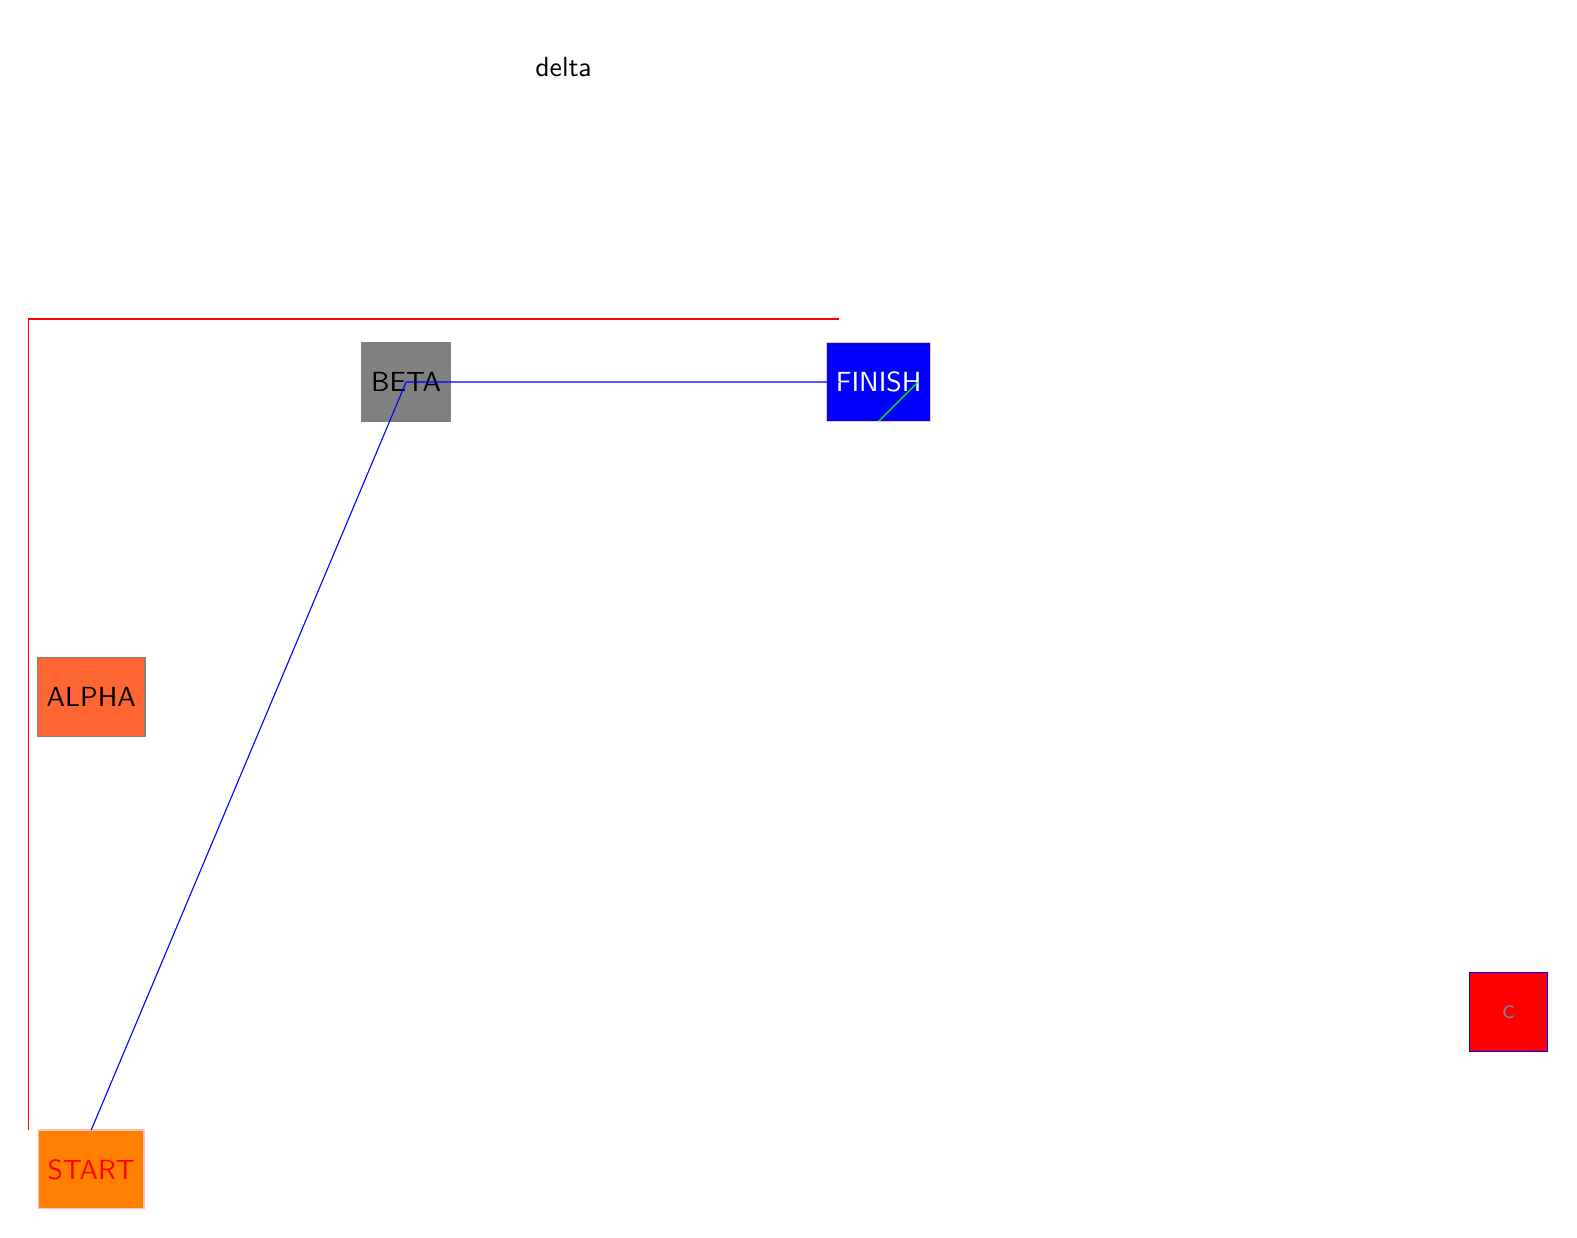
\begin{tikzpicture}
    [>={Stealth[scale=1.0]},  % Uniform arrow style
    ]
    
\node[minimum height=1cm, minimum width=1cm, fill=orange, draw=pink] (node_a) at (4,4) {\textcolor{red}{START}};
\node[minimum height=1cm, minimum width=1cm, fill=blue, draw=pink] (node_b) at (14,14) {\textcolor{white}{FINISH}};
\node[minimum height=1cm, minimum width=1cm, fill=red, draw=blue] (node_c) at (22,6) {\textcolor{gray}{c}};
\node[minimum height=1cm, minimum width=1cm, fill=colorff6633, draw=gray] (node_alpha) at (4,10) {ALPHA};
\node[minimum height=1cm, minimum width=1cm, fill=gray, draw=gray] (node_beta) at (8,14) {BETA};
\node[minimum height=1cm, minimum width=1cm] (node_delta) at (10,18) {delta};
\draw[draw=blue] (4,4.5) -- (8,14) -- (13.5,14);
\draw[draw=red] (3.2,4.5) -- (3.2,14.8) -- (13.5,14.8);
\draw[draw=green] (14.5,14) -- (14,13.5);

\end{tikzpicture}
\end{document}
